\documentclass[portuguese]{sbc2025}%

\usepackage[misc,geometry]{ifsym}

\raggedbottom  % Prevent underfull vbox warnings

\usepackage{aas_macros}
\usepackage[bottom]{footmisc}

\usepackage{tabularray}
\usepackage{adjustbox}
\usepackage{stfloats}

\usepackage{afterpage}
\usepackage{url}
\usepackage{pifont}

\setcitestyle{square}

\definecolor{engtitle}{rgb}{0.5,0.5,0.5}
\definecolor{orcidlogo}{rgb}{0.37,0.48,0.13}
\definecolor{unilogo}{rgb}{0.16, 0.26, 0.58}
\definecolor{maillogo}{rgb}{0.58, 0.16, 0.26}
\definecolor{darkblue}{rgb}{0.0,0.0,0.0}
\hypersetup{colorlinks,breaklinks,
            linkcolor=darkblue,urlcolor=darkblue,
            anchorcolor=darkblue,citecolor=darkblue}

\jyear{2025}

\category{Artigo de Pesquisa/Research Paper}
\title[Sistema de Monitoria-IC: Plataforma Web para Gestão de Monitorias Acadêmicas da UFBA]{Sistema de Monitoria-IC: Plataforma Web para Gestão Completa de Monitorias Acadêmicas da UFBA}
\engtitle{\textcolor{engtitle}{Sistema de Monitoria-IC: Web Platform for Complete Management of Academic Monitoring Programs at UFBA}}

\author[Sena et al. 2025]{
\affil{\textbf{Luis Felipe Cordeiro Sena}~\orcidlink{0009-0009-3997-3639}~\textcolor{blue}{\faEnvelopeO}~~[{Universidade Federal da Bahia}~|\href{mailto:luis.sena@ufba.br}{~{\textit{luis.sena@ufba.br}}}~]}

\affil{\textbf{Frederico Araújo Durão}~\orcidlink{0000-0002-7766-6666}~~[{Universidade Federal da Bahia}~| \href{mailto:fdurao@ufba.br}{{\textit{fdurao@ufba.br}}}~]}
}

\begin{document}

\begin{frontmatter}

\maketitle

\begin{mail}
Instituto de Computação, Universidade Federal da Bahia, Av. Milton Santos, s/n - Campus de Ondina, PAF 2, Salvador, BA, 40170-110, Brasil.
\end{mail}

\begin{abstract-pt}
A monitoria acadêmica é um processo fundamental nas universidades brasileiras que permite aos alunos desenvolverem habilidades pedagógicas enquanto auxiliam no processo de ensino-aprendizagem. Porém, o gerenciamento desse processo frequentemente enfrenta desafios relacionados à burocracia, falta de transparência e múltiplos processos manuais ineficientes. Este trabalho apresenta o desenvolvimento do Sistema de Monitoria-IC, uma plataforma web projetada para automatizar e simplificar todo o ciclo de vida dos projetos de monitoria na UFBA. A solução proposta digitaliza desde a criação de projetos pelos professores até a seleção de monitores, alocação de bolsas e geração de relatórios finais. O sistema foi desenvolvido utilizando tecnologias modernas como Next.js 15, TypeScript, tRPC, PostgreSQL e MinIO, seguindo princípios de engenharia de software que garantem escalabilidade e manutenibilidade. A arquitetura implementada separa claramente as responsabilidades entre um Sistema de Processamento de Transações (SPT) para operações cotidianas e funcionalidades gerenciais para análise e controle. A validação técnica através de testes end-to-end demonstra a robustez da solução. Os resultados indicam que a automação proposta elimina retrabalho administrativo, aumenta a transparência através de histórico auditável, e estabelece uma base sólida para modernização da gestão acadêmica na universidade. O sistema encontra-se disponível em produção em https://sistema-de-monitoria.app.ic.ufba.br/.
\end{abstract-pt}

\begin{abstract-en}
Academic monitoring is a fundamental process in Brazilian universities that allows students to develop pedagogical skills while assisting in the teaching-learning process. However, managing this process often faces challenges related to bureaucracy, lack of transparency, and multiple inefficient manual procedures. This work presents the development of Sistema de Monitoria-IC, a web platform designed to automate and simplify the entire lifecycle of monitoring projects at UFBA. The proposed solution digitizes everything from project creation by professors to monitor selection, scholarship allocation, and final report generation. The system was developed using modern technologies such as Next.js 15, TypeScript, tRPC, PostgreSQL, and MinIO, following software engineering principles that ensure scalability and maintainability. The implemented architecture clearly separates responsibilities between a Transaction Processing System (TPS) for daily operations and managerial functionalities for analysis and control. Technical validation through end-to-end tests demonstrates the solution's robustness. Results indicate that the proposed automation eliminates administrative rework, increases transparency through auditable history, and establishes a solid foundation for modernizing academic management at the university. The system is available in production at https://sistema-de-monitoria.app.ic.ufba.br/.
\end{abstract-en}

\begin{pchaves}
Gestão Acadêmica, Sistema de Monitoria, Arquitetura de Software, Desenvolvimento Web, Automação de Processos.
\end{pchaves}

\begin{keywords}
Academic Management, Monitoring System, Software Architecture, Web Development, Process Automation.
\end{keywords}

\begin{dates}
% Informações serão preenchidas pelo editor antes da publicação
\end{dates}

\end{frontmatter}

\section{Introdução}
\label{sec:intro}

\subsection{Contextualização e Motivação}

A monitoria acadêmica representa um dos pilares fundamentais do ensino superior brasileiro, estabelecendo-se como uma prática pedagógica que beneficia simultaneamente monitores, estudantes e docentes. Regulamentada pela Lei nº 9.394/96 (Lei de Diretrizes e Bases da Educação Nacional), a monitoria permite que alunos com destacado desempenho acadêmico auxiliem seus pares no processo de aprendizagem, desenvolvendo competências didáticas enquanto aprofundam seus conhecimentos na disciplina \cite{Brasil1996}.

Na Universidade Federal da Bahia (UFBA), o programa de monitoria segue um fluxo complexo que envolve múltiplos atores e etapas interdependentes. O processo inicia-se com o planejamento semestral, quando a administração importa dados de disciplinas e professores. Em seguida, os docentes criam e submetem projetos de monitoria que precisam ser aprovados administrativamente. Após a aprovação, ocorre a publicação de editais internos, inscrição de candidatos, processo seletivo, alocação de bolsas, e finalmente, a consolidação de dados para envio à PROGRAD (Pró-Reitoria de Graduação).

A literatura de Sistemas de Informação fornece evidências de que a digitalização e a automação de processos reduzem custos transacionais, eliminam retrabalho e aumentam a confiabilidade e a auditabilidade dos registros \cite{Laudon_Laudon_2011, Davenport1993, Hammer1993}. Em contextos públicos e acadêmicos, iniciativas de governo digital e transformação digital têm sido associadas a ganhos de eficiência administrativa e transparência, desde que apoiadas por arquitetura tecnológica moderna e governança de dados adequada \cite{OECD2020, UNESCO2022}. No escopo deste trabalho, adotamos tais fundamentos para sustentar a proposta de um sistema unificado de monitoria, substituindo fluxos fragmentados por um \textit{workflow} padronizado, rastreável e escalável.

Apesar de sua importância reconhecida, a gestão dos programas de monitoria na UFBA ainda depende predominantemente de processos manuais e fragmentados. Formulários em papel, planilhas eletrônicas dispersas, comunicação via e-mail e ausência de um sistema centralizado caracterizam o cenário atual, resultando em ineficiências operacionais significativas. Essa realidade contrasta com a tendência global de digitalização e automação de processos administrativos no ambiente acadêmico, conforme defendem \cite{Laudon_Laudon_2011}, que argumentam que a tecnologia da informação constitui uma das principais ferramentas para alcançar excelência operacional.

\subsection{Identificação do Problema}

O processo tradicional de gestão de monitoria apresenta gargalos que afetam professores, estudantes e administração. Do ponto de vista docente, grande parte do tempo é consumida em rotinas burocráticas repetitivas e na reescrita de projetos que poderiam aproveitar modelos de semestres anteriores. A etapa de seleção tende a ser morosa pela análise manual de documentos, e faltam mecanismos padronizados para acompanhar atividades e consolidar relatórios ao fim do período.

Para os estudantes, a experiência também é fragmentada: a descoberta de oportunidades depende de canais dispersos, as inscrições frequentemente exigem múltiplos formulários e anexos enviados por meios distintos, e a ausência de um painel unificado dificulta o acompanhamento de prazos, resultados e do próprio histórico de participação.

Na esfera administrativa, o cenário é marcado por retrabalho na consolidação de dados oriundos de fontes heterogêneas, por dificuldades para assegurar conformidade com prazos e regulamentos e pela inexistência de uma base de dados integrada que apoie planejamento, prestação de contas e análises históricas. A elaboração de relatórios para órgãos superiores consome esforço manual considerável e é suscetível a falhas de transcrição.

Em síntese, há uma lacuna tecnológica clara: falta um sistema de informação \textit{fim-a-fim} específico para monitoria que integre criação de projetos, aprovação administrativa, publicação de editais, inscrições, seleção e consolidações finais. Ao unificar o processo, espera-se um impacto positivo mensurável -- redução de tempo de processamento, diminuição de erros, transparência com histórico auditável e melhor suporte a decisões -- em linha com a evidência da literatura sobre reengenharia de processos e sistemas gerenciais \cite{Davenport1993, Hammer1993, Laudon_Laudon_2011}.

\subsection{Objetivos}

Este trabalho documenta o desenvolvimento e implementação do \textbf{Sistema de Monitoria-IC}, uma plataforma web completa para gestão dos projetos de monitoria do Instituto de Computação da UFBA. O objetivo central é substituir fluxos manuais e dispersos por um sistema único que garanta transparência, rastreabilidade e padronização de todo o processo de monitoria.

Os objetivos específicos incluem:

\begin{enumerate}
  \item \textbf{Digitalizar o ciclo completo de projetos de monitoria:} desde a criação com templates reutilizáveis, assinatura digital pelo professor, submissão, até aprovação administrativa e publicação de editais

  \item \textbf{Automatizar o processo seletivo:} permitindo inscrições online, captura automática de notas e CR do histórico, consideração de equivalências entre disciplinas, e publicação transparente de resultados

  \item \textbf{Sistematizar a alocação de bolsas:} com geração automática de planilhas para o Instituto, configuração do total de bolsas informado pela PROGRAD, e alocação por projeto com validações automáticas

  \item \textbf{Eliminar trabalhos manuais repetitivos:} através de automação de notificações por e-mail, geração de documentos PDF, e integração com armazenamento de arquivos

  \item \textbf{Fornecer base analítica para tomada de decisões:} com dashboards administrativos, APIs para integração, e relatórios consolidados para análises institucionais
\end{enumerate}

% (Subseção removida para reduzir subdivisão e privilegiar narrativa contínua.)
Este artigo está organizado da seguinte forma: a Seção 2 apresenta os fundamentos teóricos sobre Sistemas de Informação e monitoria acadêmica. A Seção 3 analisa trabalhos relacionados e o estado da prática em universidades brasileiras. A Seção 4 detalha a arquitetura, tecnologias e implementação do Sistema de Monitoria-IC. A Seção 5 apresenta os resultados obtidos e discussões. Por fim, a Seção 6 conclui o trabalho e aponta direções futuras.

\section{Fundamentação Teórica}
\label{sec:background}

\subsection{Monitoria Acadêmica no Ensino Superior Brasileiro}

A monitoria acadêmica constitui uma modalidade de ensino-aprendizagem que contribui para a formação integrada do aluno nas atividades de ensino, pesquisa e extensão dos cursos de graduação. Conforme estabelecido pela Lei de Diretrizes e Bases da Educação Nacional (Lei nº 9.394/96), as universidades devem aproveitar estudantes de bom rendimento acadêmico em tarefas de ensino e pesquisa \cite{Brasil1996}.

O processo de monitoria na UFBA segue diretrizes institucionais que estabelecem critérios de seleção baseados no desempenho acadêmico (nota na disciplina e Coeficiente de Rendimento), definem modalidades de participação (bolsista e voluntário), delimitam responsabilidades de monitores, professores e coordenação, regulam o fluxo de aprovação de projetos e alocação de recursos e definem requisitos de certificação ao final do período.

Estudos sobre programas de monitoria demonstram benefícios significativos: desenvolvimento de habilidades didáticas nos monitores \cite{Natario2010}, melhoria no desempenho acadêmico dos estudantes assistidos \cite{Frison2016}, e apoio essencial aos docentes na condução de atividades práticas \cite{Dantas2014}. Entretanto, esses mesmos estudos apontam desafios na gestão administrativa desses programas, especialmente relacionados à burocracia e falta de ferramentas adequadas.

\subsection{Sistemas de Informação na Gestão Acadêmica}

\subsubsection{Sistemas de Processamento de Transações (SPT)}

Conforme \cite{Laudon_Laudon_2011}, os SPTs são "sistemas informatizados que realizam e registram as transações rotineiras necessárias ao funcionamento organizacional". No contexto acadêmico, esses sistemas gerenciam operações como matrículas, lançamento de notas, controle de frequência e, no caso específico deste trabalho, o ciclo de vida dos projetos de monitoria.

As características essenciais de um SPT incluem alta precisão e confiabilidade dos dados, processamento eficiente de grandes volumes transacionais, mecanismos de auditoria e rastreabilidade, além de alta disponibilidade para sustentar operações críticas.

\subsubsection{Sistemas de Informações Gerenciais (SIG)}

Os SIGs, segundo \cite{Laudon_Laudon_2011}, "resumem e relatam as operações básicas da empresa usando dados fornecidos pelos SPTs". No Sistema de Monitoria-IC, o componente SIG materializa-se em painéis e relatórios consolidados que permitem monitorar o andamento dos processos, analisar tendências históricas, avaliar a distribuição de recursos entre departamentos e gerar documentos formais para órgãos superiores.

\subsubsection{Arquitetura Híbrida SPT-SIG}

A separação de responsabilidades entre SPT (camada operacional) e SIG (camada analítica) fundamenta a arquitetura do Sistema de Monitoria-IC. O SPT gerencia o ciclo de vida de cada transação – cadastros, aprovações, inscrições – enquanto o SIG consome os registros consolidados para gerar análises e relatórios. Essa divisão favorece escalabilidade independente, facilita manutenção e evolução, reduz o acoplamento entre operações e análises e permite otimizações específicas de desempenho em cada camada.

\subsection{Tecnologias Modernas para Desenvolvimento Web}

O desenvolvimento de aplicações web modernas beneficia-se de frameworks e ferramentas que promovem produtividade, manutenibilidade e desempenho. As principais tecnologias utilizadas neste projeto incluem:

\textbf{Next.js e React:} Framework full-stack que combina renderização no servidor (SSR) e no cliente (CSR), otimizando desempenho e SEO enquanto mantém a reatividade característica de Single Page Applications \cite{Vercel2024}.

\textbf{TypeScript:} Superset tipado de JavaScript que adiciona verificação estática de tipos, reduzindo erros em tempo de execução e melhorando a manutenibilidade do código \cite{Microsoft2024}.

\textbf{tRPC:} Biblioteca que permite criar APIs type-safe sem necessidade de geração de código ou schemas compartilhados, garantindo consistência entre cliente e servidor \cite{TRPC2024}.

\textbf{PostgreSQL e Drizzle ORM:} Banco de dados relacional robusto combinado com um ORM TypeScript-first que oferece type safety e migrações automáticas \cite{PostgreSQL2024, Drizzle2024}.

\section{Trabalhos Relacionados}
\label{sec:related-work}

\subsection{Sistemas de Gestão Acadêmica Generalistas}

Diversos sistemas de gestão acadêmica são utilizados em universidades brasileiras, como o SIGAA (Sistema Integrado de Gestão de Atividades Acadêmicas) desenvolvido pela UFRN e adotado por várias instituições federais \cite{UFRN2024}. Embora esses sistemas ofereçam módulos abrangentes para gestão universitária, frequentemente carecem de funcionalidades específicas para o workflow detalhado de programas de monitoria.

O SIGA (Sistema Integrado de Gestão Acadêmica) da UFRJ e o Sistema Acadêmico da USP (Júpiter) são outros exemplos de soluções institucionais que, apesar de robustas, não cobrem adequadamente funcionalidades específicas da monitoria, como o uso de templates reutilizáveis de projetos, a assinatura digital por papéis (professor e chefe de departamento), a seleção com critérios configuráveis por projeto, a consideração automática de equivalências entre disciplinas e a geração de consolidações específicas para a PROGRAD.

\subsection{Levantamento do Estado da Prática}

Para avaliar o estado atual da gestão de monitoria em universidades brasileiras, realizamos um levantamento nos cursos de Computação das dez universidades públicas mais bem classificadas segundo o Ranking Universitário Folha (RUF) 2024 \cite{folha2024ruf}.

\begin{table*}[htb]
  \centering
\caption{Panorama da gestão de monitoria em universidades públicas brasileiras.\\Fonte: páginas oficiais dos sistemas institucionais Júpiter/USP \cite{USPJupiter}, SIGA/UFRJ \cite{UFRJ_SIGA}, SIGAA/UnB \cite{UnB_SIGAA}, CAGR/UFSC \cite{UFSC_CAGR} e SEI/UNIFESP \cite{UNIFESP_SEI}; complementado por análise de editais e orientações públicas (2024--2025).}
  \label{tab:estado-pratica}
  \begin{adjustbox}{max width=\textwidth}
    \begin{tabular}{|c|l|c|c|p{3cm}|p{5cm}|}
      \hline
      \textbf{Rank} & \textbf{Universidade} & \textbf{Sistema Específico} & \textbf{Sistema Integrado} & \textbf{Ferramentas} & \textbf{Características} \\
      \hline
      1º & USP & Não & Parcial & Júpiter + Forms & Cadastro no sistema acadêmico, seleção via formulários \\
      \hline
      2º & Unicamp & Não & Não & E-mail + Planilhas & Processo totalmente manual \\
      \hline
      3º & UFRGS & Não & Sim & Portal do Aluno & Funcionalidades básicas no portal institucional \\
      \hline
      4º & UFRJ & Não & Parcial & SIGA + E-mail & Registro no SIGA, processo seletivo manual \\
      \hline
      5º & UFMG & Não & Não & Google Forms & Inscrições via formulários, gestão em planilhas \\
      \hline
      6º & UNESP & Não & Não & E-mail + Docs & Processo manual com documentos Word \\
      \hline
      7º & UFSC & Não & Sim & CAGR & Sistema acadêmico com módulo básico \\
      \hline
      8º & UnB & Não & Parcial & SIGAA & Módulo genérico no SIGAA \\
      \hline
      9º & UNIFESP & Não & Não & SEI + Forms & Processo administrativo via SEI \\
      \hline
      10º & UFPR & Não & Não & Microsoft Forms & Formulários online, gestão manual \\
      \hline
    \end{tabular}
  \end{adjustbox}
\end{table*}

\noindent\textit{Fonte e metodologia do levantamento.} Panorama elaborado a partir de páginas oficiais dos sistemas institucionais: Júpiter (USP) \cite{USPJupiter}, SIGA (UFRJ) \cite{UFRJ_SIGA}, SIGAA (UnB) \cite{UnB_SIGAA}, CAGR (UFSC) \cite{UFSC_CAGR} e SEI (UNIFESP) \cite{UNIFESP_SEI}. Para as instituições sem sistema específico de monitoria, a classificação decorre da análise de editais e orientações públicas de 2024--2025, os quais indicam processos manuais com formulários e planilhas.

Os resultados revelam que nenhuma instituição analisada dispõe de um sistema específico e completo para gestão de monitoria; cerca de 70\% recorrem a ferramentas genéricas (Google/Microsoft Forms e e-mail) e apenas 30\% apresentam algum nível de integração com sistemas acadêmicos. Em todos os casos foram observadas etapas manuais significativas nos processos seletivos e ausência de padronização ou compartilhamento de soluções entre instituições.

\subsection{Análise Comparativa}

A análise dos trabalhos relacionados e do estado da prática revela uma lacuna significativa: enquanto há sistemas acadêmicos robustos para gestão geral, falta uma solução que trate as particularidades da monitoria. O Sistema de Monitoria-IC distingue-se por ser específico para o \textit{workflow} de monitoria, cobrir o ciclo de vida completo (da criação de projetos à emissão de certificados), automatizar etapas via integrações e processamento inteligente, adotar um \textit{stack} moderno com foco em experiência do usuário e desempenho e, sobretudo, garantir transparência com rastreabilidade e acesso diferenciado por papéis.

\section{Sistema de Monitoria-IC}
\label{sec:system}

\subsection{Visão Geral da Arquitetura}

O Sistema de Monitoria-IC foi projetado seguindo uma arquitetura em camadas que separa claramente as responsabilidades e promove manutenibilidade e escalabilidade. A arquitetura segue o padrão de três camadas com componentes especializados:

\subsubsection{Camada de Apresentação}

Implementada como uma Single Page Application (SPA) usando Next.js 15, React e TypeScript, com interface responsiva construída a partir de componentes shadcn/ui e Tailwind CSS. O roteamento é dinâmico e protegido por papéis, o estado do cliente é coordenado por React Query e Zustand e os formulários utilizam React Hook Form com validações em Zod.

\subsubsection{Camada de Aplicação}

A camada de aplicação utiliza tRPC v11 para prover uma API \textit{type-safe} entre cliente e servidor. As procedures são organizadas por domínio (projeto, inscrição, edital, entre outros), com autenticação via Lucia Auth, validações automáticas com Zod e suporte a \textit{subscriptions} para atualizações em tempo quase real.

\subsubsection{Camada de Negócio}

A camada de negócio concentra serviços especializados: o \texttt{ProjectService} gerencia o ciclo de vida de projetos, o \texttt{SelectionService} processa inscrições e seleções, o \texttt{NotificationService} orquestra notificações por e-mail, o \texttt{DocumentService} cuida da geração de PDFs e das assinaturas e o \texttt{AnalyticsService} consolida dados para relatórios e painéis.

\subsubsection{Camada de Dados}

A camada de dados utiliza PostgreSQL com Drizzle ORM para persistência e MinIO para armazenamento de objetos. O esquema é relacional e normalizado, com integridade referencial e migrações versionadas e reversíveis; índices otimizam consultas frequentes, enquanto rotinas de backup e replicação asseguram resiliência.

\subsection{Modelo de Dados}

O modelo de dados foi projetado para capturar todas as entidades e relacionamentos do domínio de monitoria, seguindo princípios de normalização e integridade referencial. As principais entidades e seus relacionamentos são apresentados a seguir:

No núcleo de usuários, a entidade \texttt{user} concentra autenticação e perfil básico, estendida por perfis específicos de \texttt{professor} (dados acadêmicos) e \texttt{aluno} (matrícula, curso e CR), com papéis representados por \texttt{role} (\textit{admin}, \textit{professor}, \textit{student}). No eixo acadêmico, \texttt{departamento}, \texttt{curso}, \texttt{disciplina} e \texttt{periodo} descrevem a hierarquia institucional, os cursos vinculados, as disciplinas (com códigos e equivalências) e os semestres letivos. No domínio da monitoria, \texttt{projeto} evolui por estados bem definidos (DRAFT, SUBMITTED, APPROVED) e se relaciona a \texttt{projeto\_template} para reuso; \texttt{edital} organiza publicações por período; \texttt{inscricao} registra candidaturas e notas; \texttt{vaga} modela posições de monitor (BOLSISTA, VOLUNTARIO); e \texttt{documento} centraliza arquivos e assinaturas digitais.

\subsection{Fluxo de Processos}

O fluxo de monitoria é orquestrado em seis etapas contínuas que estruturam o semestre. Na fase de planejamento e criação, a administração importa a planilha institucional de disciplinas e professores (SIAPE); o sistema identifica projetos individuais e coletivos, gera versões iniciais com base em templates de semestres anteriores e notifica docentes para revisão, edição e assinatura digital. Em seguida, ocorre a aprovação administrativa: projetos submetidos são avaliados com feedback, e a consolidação aprovada resulta em planilha com links em PDF encaminhada ao Instituto para viabilizar a solicitação de bolsas.

Com a definição do total de bolsas pela PROGRAD, inicia-se a alocação e a publicação do edital interno. O sistema impede excedentes na distribuição, permite que professores configurem vagas de voluntariado e conduz a geração do edital com assinatura digital do chefe de departamento, finalizando com publicação e notificações automáticas. A fase de inscrições e seleção disponibiliza um catálogo de vagas para os estudantes; o sistema captura automaticamente CR e notas (respeitando equivalências configuradas), enquanto os docentes avaliam candidatos e publicam resultados, contemplando bolsistas e voluntários.

Após a seleção, a etapa de aceite e consolidação final confirma as vagas: estudantes aceitam ou rejeitam convites, bolsistas informam dados bancários e a administração valida requisitos pendentes. O sistema produz a planilha final para a PROGRAD, encaminhada via Departamento. Por fim, o encerramento do ciclo envolve relatórios e certificados: os professores geram o relatório final da disciplina, os relatórios individuais dos monitores são assinados digitalmente (professor e aluno), a ata departamental é consolidada e são emitidos certificados para encaminhamento ao NUMOP.

\subsection{Implementação e Tecnologias}

\subsubsection{Stack Tecnológico}

O sistema utiliza tecnologias modernas e consolidadas:

No \textit{frontend}, o sistema adota Next.js 15.1.4 (App Router) com TypeScript 5.x para \textit{type safety}. A interface utiliza Tailwind CSS e shadcn/ui; os formulários são implementados com React Hook Form e Zod; a sincronização de estado remoto e o cache são tratados por React Query. No \textit{backend}, a API \textit{type-safe} é construída com tRPC v11 e protegida por Lucia Auth; a persistência usa Drizzle ORM com PostgreSQL; documentos são armazenados no MinIO (S3-compatible) e o envio de e-mails é realizado via Nodemailer. Em \textit{DevOps}, a solução é containerizada com Docker e validada por uma pipeline no GitHub Actions que executa linting (Biome), verificação de tipos, testes unitários (Vitest), testes E2E (Playwright) e build de produção.

\subsubsection{Principais Routers tRPC}

O sistema organiza a lógica de negócio em routers especializados:

\begin{verbatim}
// src/server/api/root.ts
export const appRouter = createTRPCRouter({
  // Autenticação e usuários
  auth: authRouter,
  me: meRouter,
  user: userRouter,
  apiKey: apiKeyRouter,

  // Entidades acadêmicas
  departamento: departamentoRouter,
  curso: courseRouter,
  discipline: disciplineRouter,

  // Gestão de monitoria
  projeto: projetoRouter,
  projetoTemplates: projetoTemplatesRouter,
  edital: editalRouter,
  inscricao: inscricaoRouter,
  selecao: selecaoRouter,
  vagas: vagasRouter,

  // Administrativo
  importProjects: importProjectsRouter,
  scholarshipAllocation: scholarshipRouter,
  analytics: analyticsRouter,
  relatorios: relatoriosRouter,

  // Infraestrutura
  file: fileRouter,
  signature: signatureRouter,
  notificacoes: notificacoesRouter,
});
\end{verbatim}

\subsection{Funcionalidades Implementadas}

A Tabela \ref{tab:funcionalidades} apresenta o status atual das funcionalidades do sistema:

\begin{table*}[htb]
  \centering
  \caption{Funcionalidades implementadas no Sistema de Monitoria-IC}
  \label{tab:funcionalidades}
  \begin{tabular}{|l|p{9cm}|}
    \hline
    \textbf{Funcionalidade} & \textbf{Descrição} \\
    \hline
    Importação de planejamento & Parser de Excel para importação de disciplinas e professores, criação automática de projetos individuais e coletivos \\
    \hline
    Templates de projetos & Sistema de templates reutilizáveis entre semestres, reduzindo tempo de criação \\
    \hline
    Assinatura digital & Integração completa com serviço de assinatura eletrônica para professores e chefe de departamento \\
    \hline
    Workflow de aprovação & Estados bem definidos (DRAFT, SUBMITTED, APPROVED) com notificações automáticas \\
    \hline
    Geração de editais & Criação automática de PDF do edital interno com assinatura digital do chefe \\
    \hline
    Alocação de bolsas & Sistema inteligente com validação de limites e distribuição otimizada \\
    \hline
    Inscrições online & Portal completo para candidatos com upload de documentos e acompanhamento \\
    \hline
    Captura de dados acadêmicos & Integração parcial com sistema acadêmico para notas e CR \\
    \hline
    Equivalências de disciplinas & Sistema configurável para considerar disciplinas equivalentes na seleção \\
    \hline
    Seleção de monitores & Interface completa para professores avaliarem e selecionarem candidatos \\
    \hline
    Aceite de vagas & Portal para alunos aceitarem/rejeitarem vagas com coleta de dados bancários \\
    \hline
    Relatórios & Geração de relatórios parciais e consolidações para PROGRAD \\
    \hline
    Certificados & Módulo em desenvolvimento para emissão automática \\
    \hline
    Dashboard analytics & Painel completo com métricas em tempo real e visualizações interativas \\
    \hline
    API de integração & Endpoints REST e tRPC para integração com sistemas externos \\
    \hline
  \end{tabular}
\end{table*}

\subsection{Interfaces do Sistema}

As figuras a seguir apresentam as principais telas do sistema em produção:

\begin{figure}[h!]
  \centering
  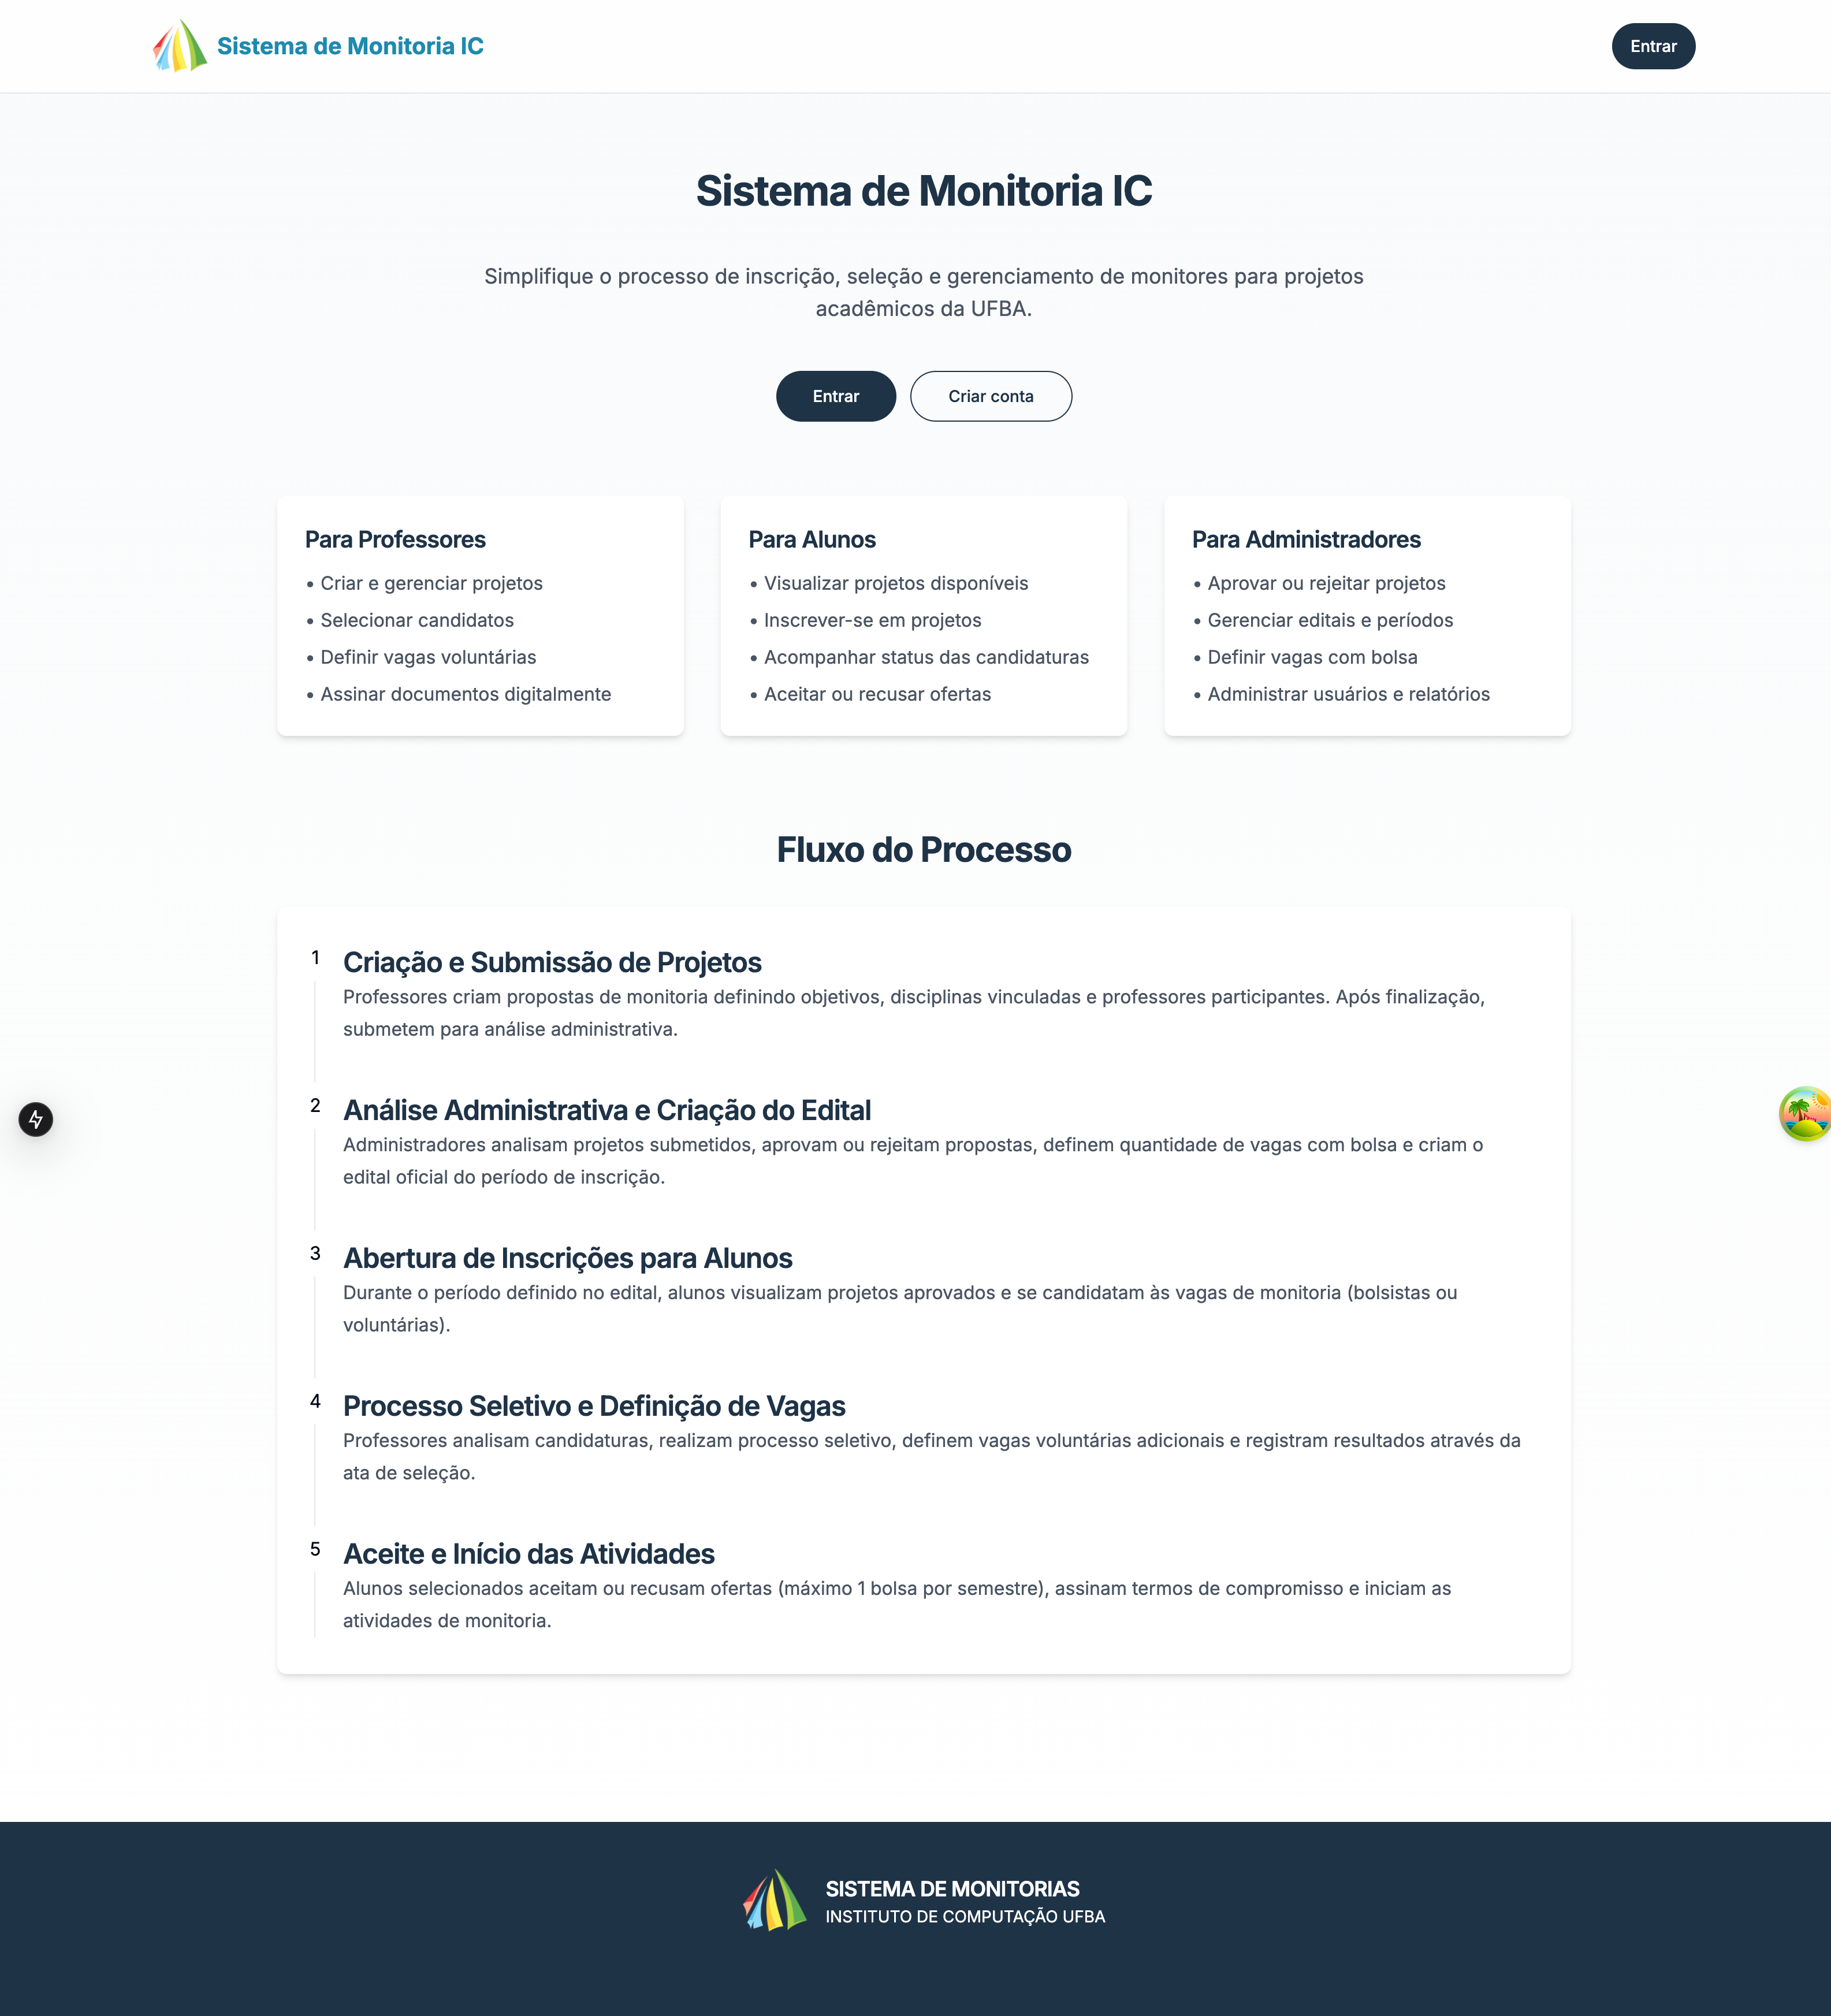
\includegraphics[width=\linewidth]{images/monitoria/landing.png}
  \caption{Página inicial pública do sistema}
  \label{fig:landing}
\end{figure}

\begin{figure}[h!]
  \centering
  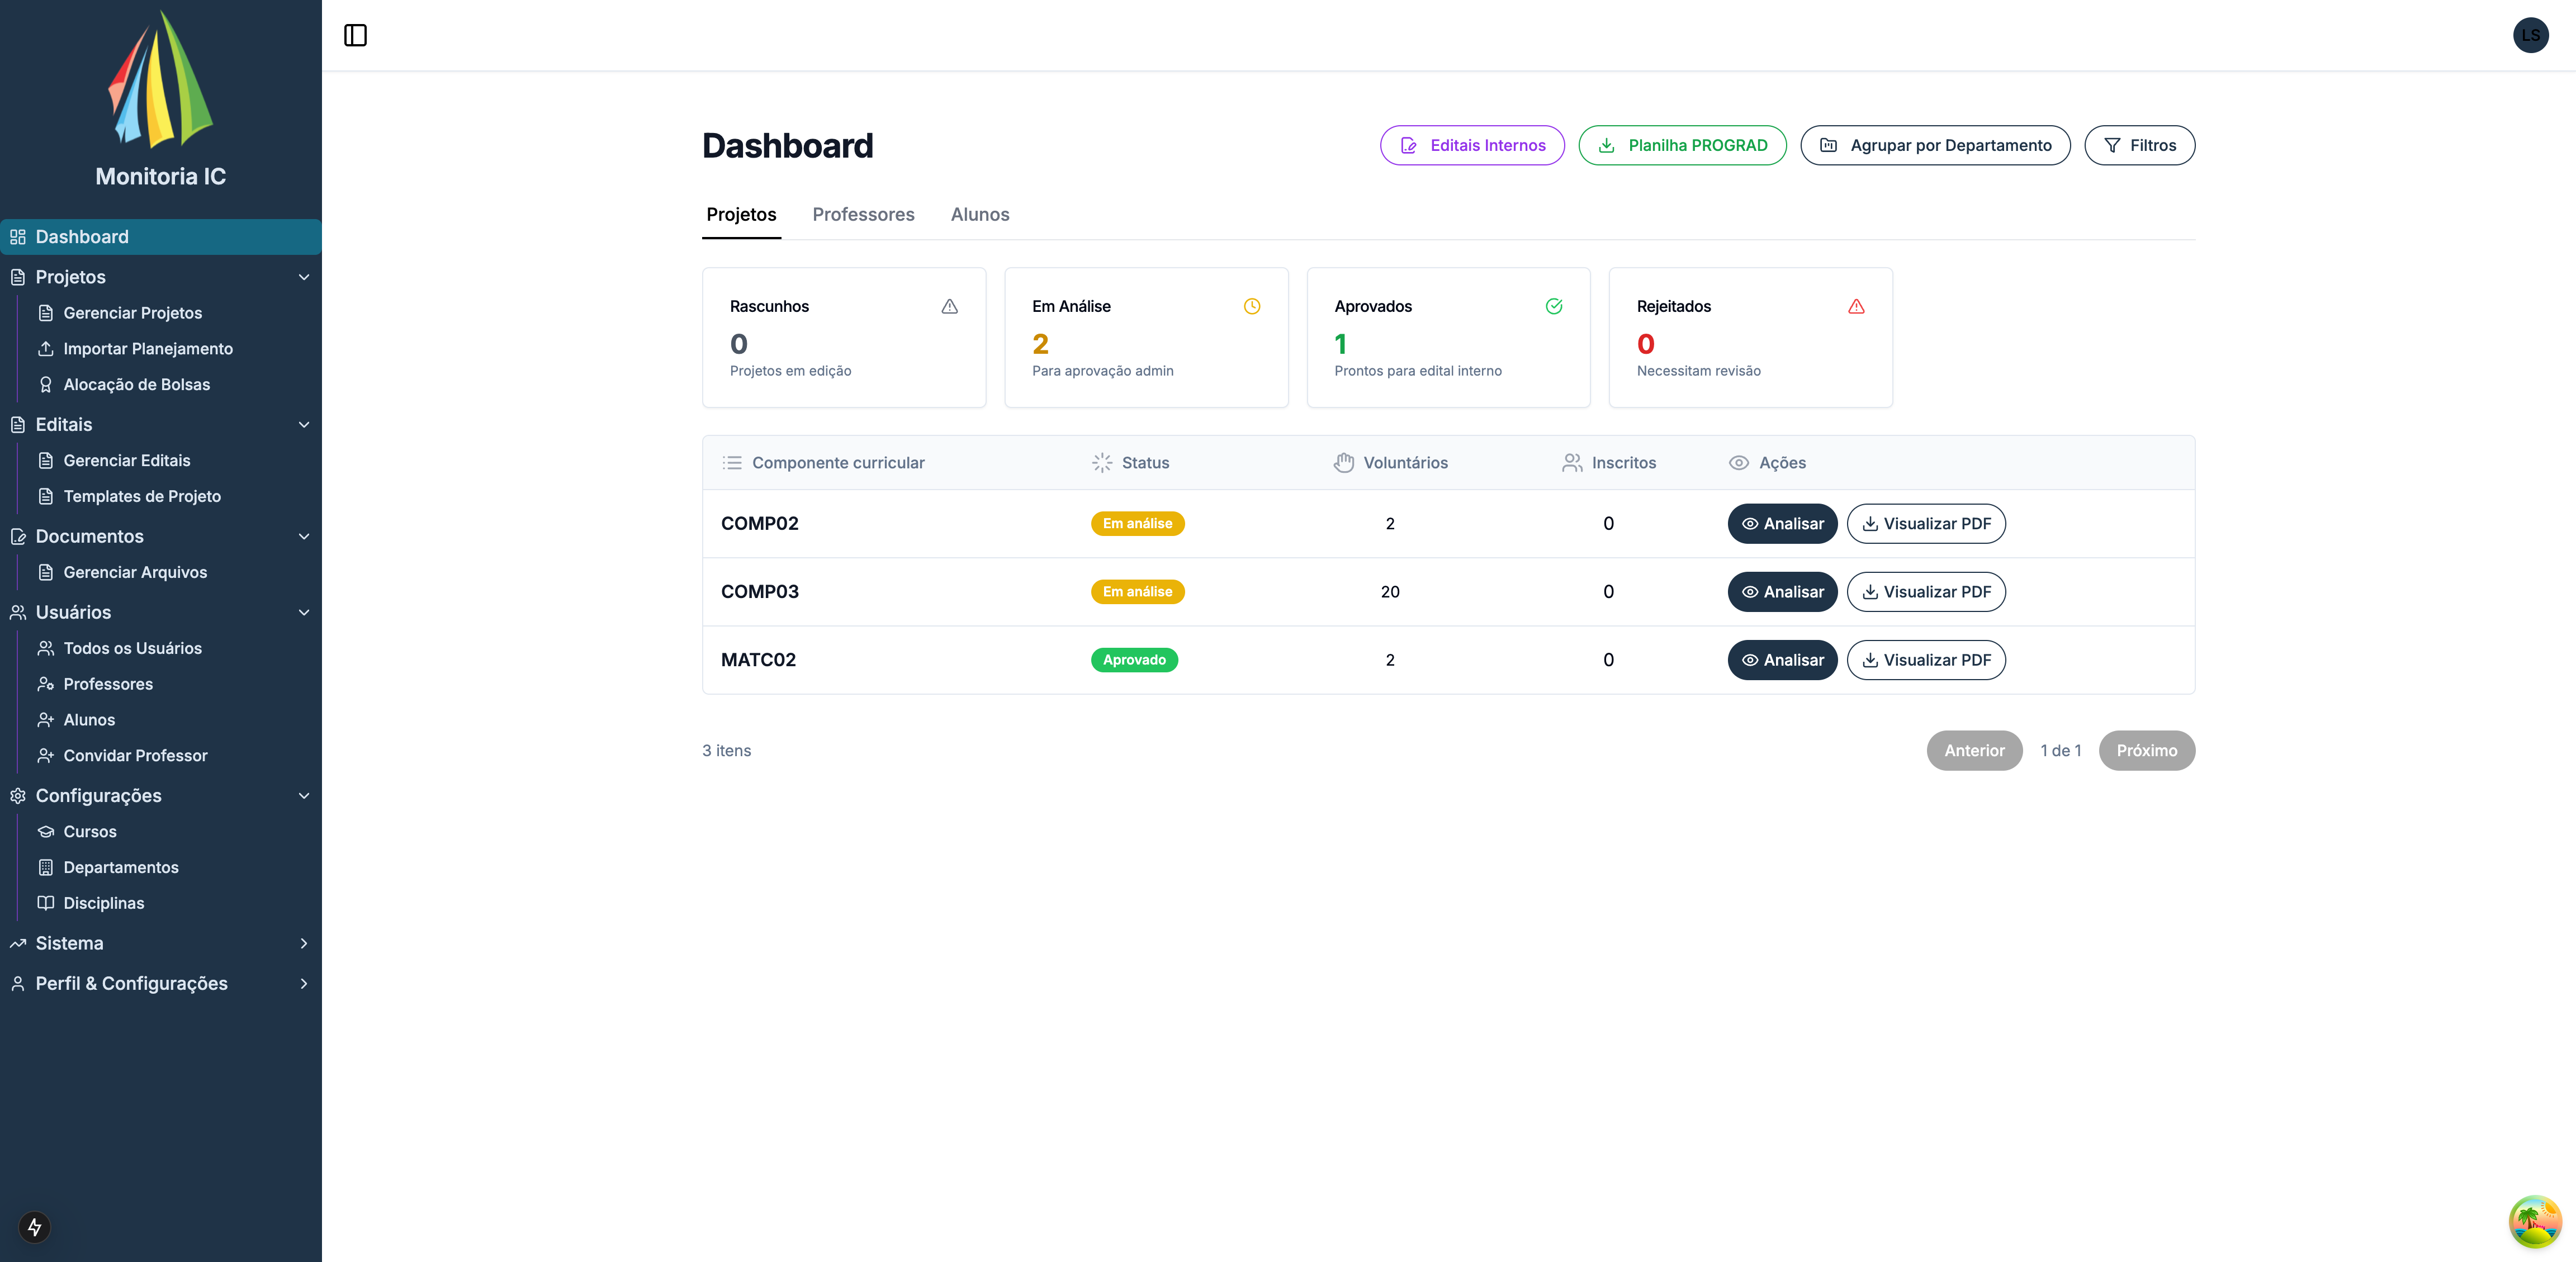
\includegraphics[width=\linewidth]{images/monitoria/admin-dashboard.png}
  \caption{Dashboard administrativo com métricas}
  \label{fig:dashboard}
\end{figure}

\begin{figure}[h!]
  \centering
  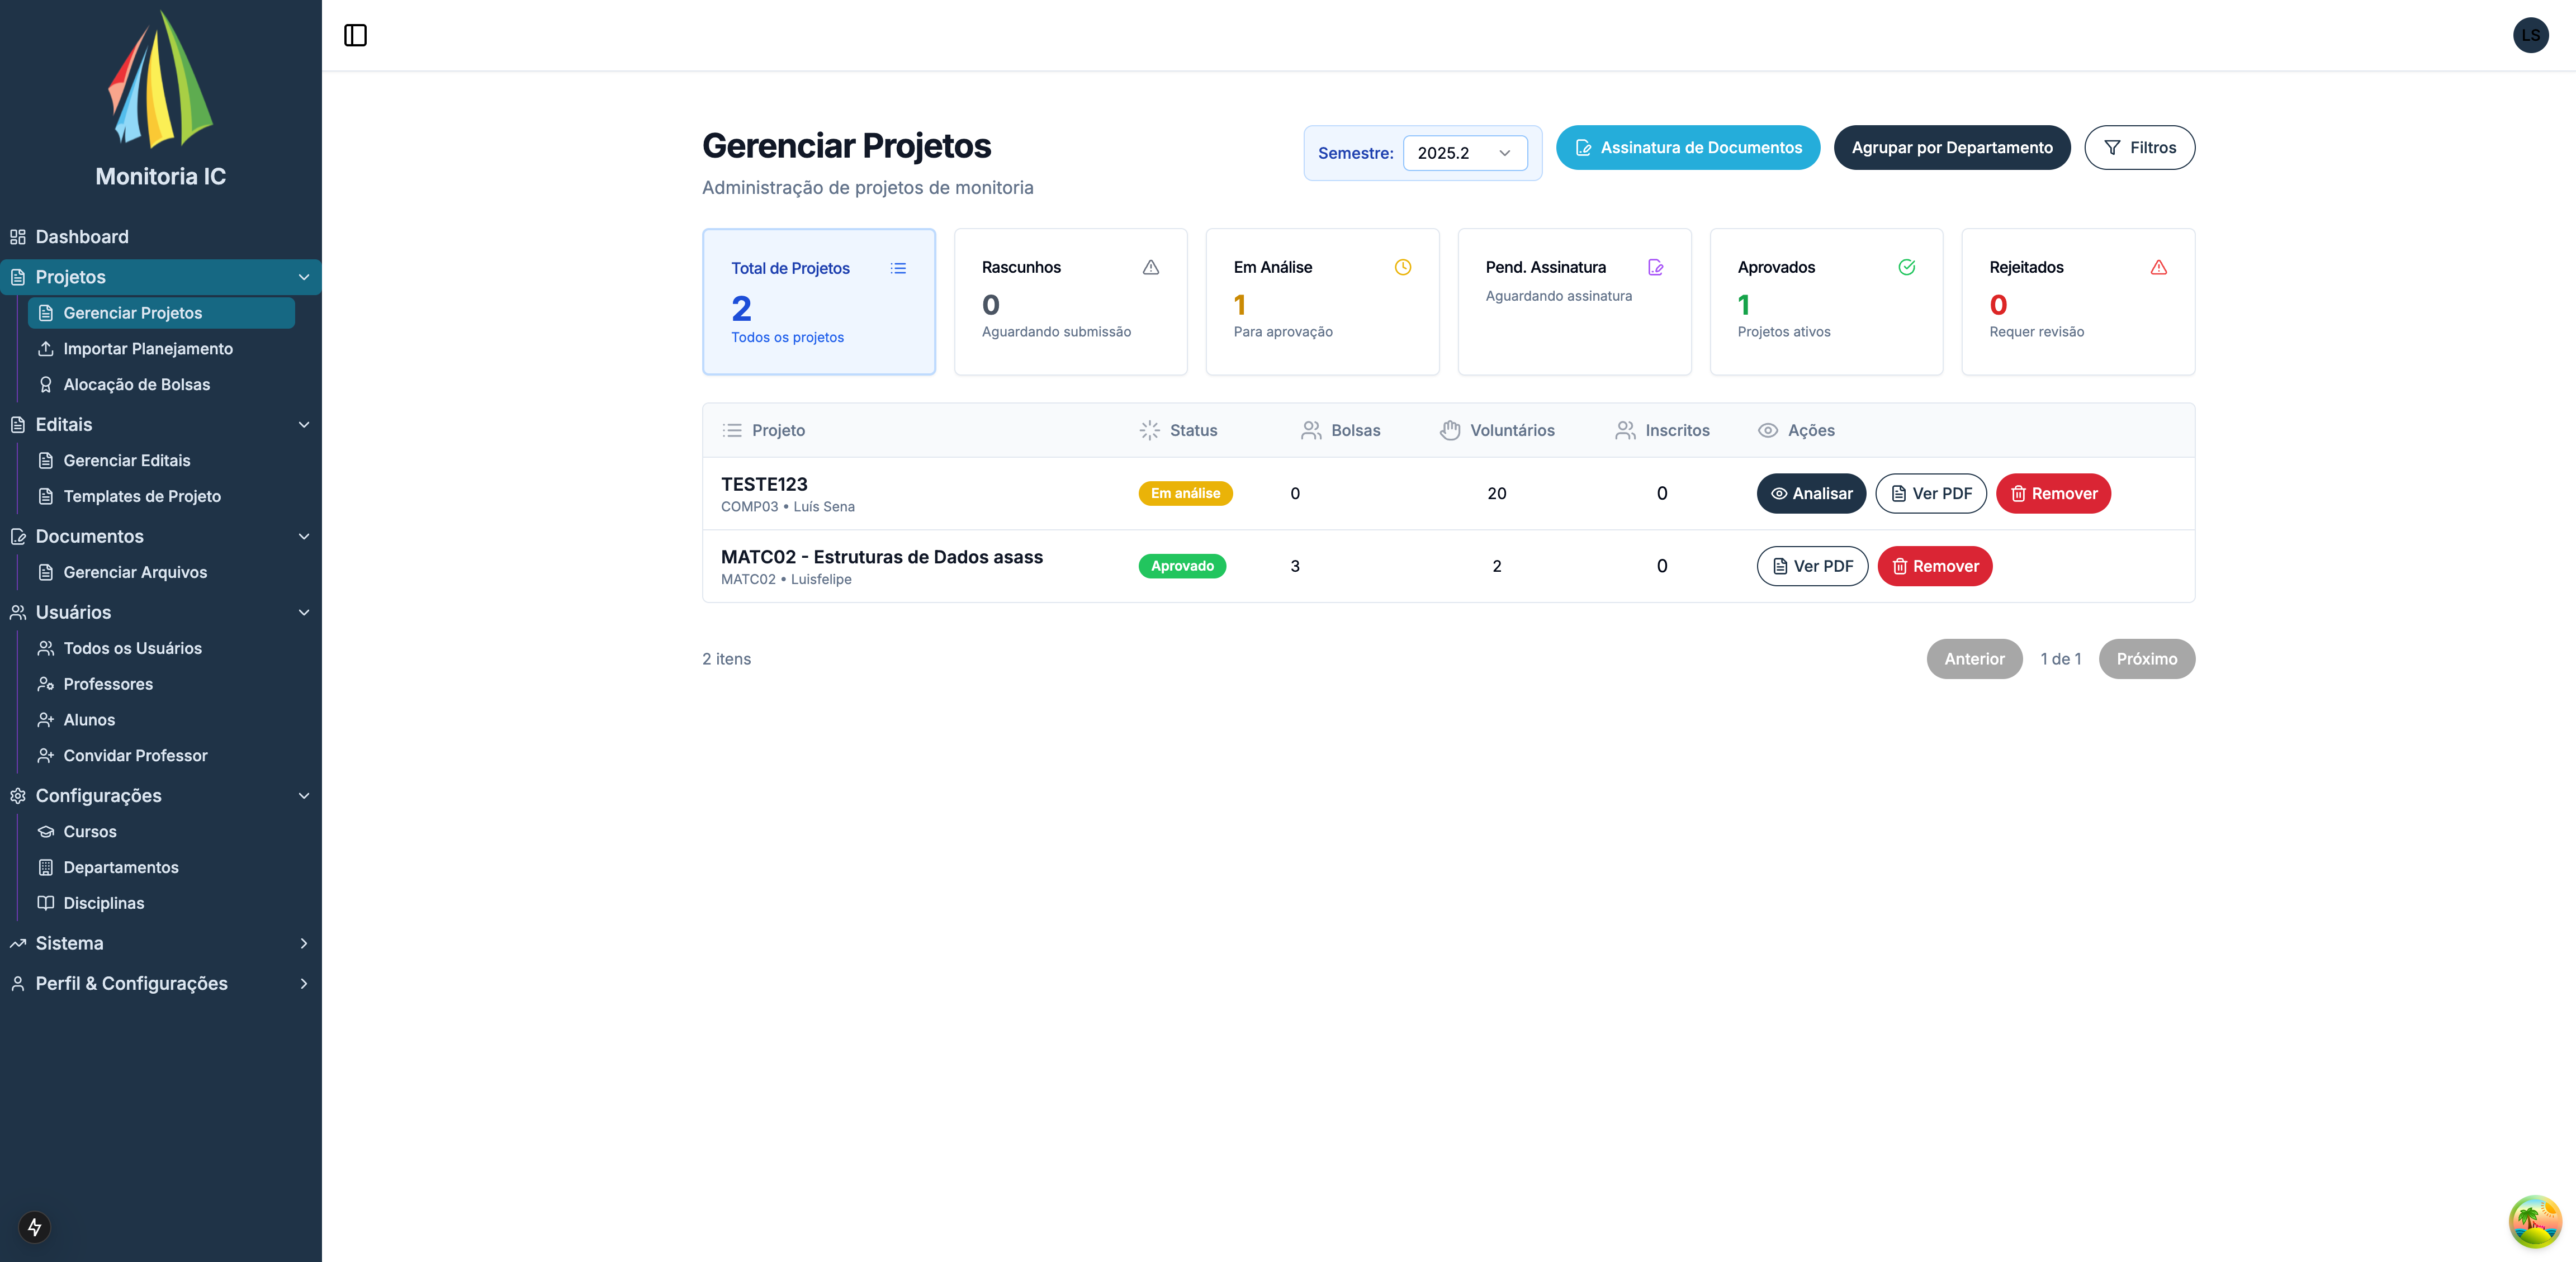
\includegraphics[width=\linewidth]{images/monitoria/admin-manage-projects.png}
  \caption{Gerenciamento de projetos por semestre}
  \label{fig:projetos}
\end{figure}

\begin{figure}[h!]
  \centering
  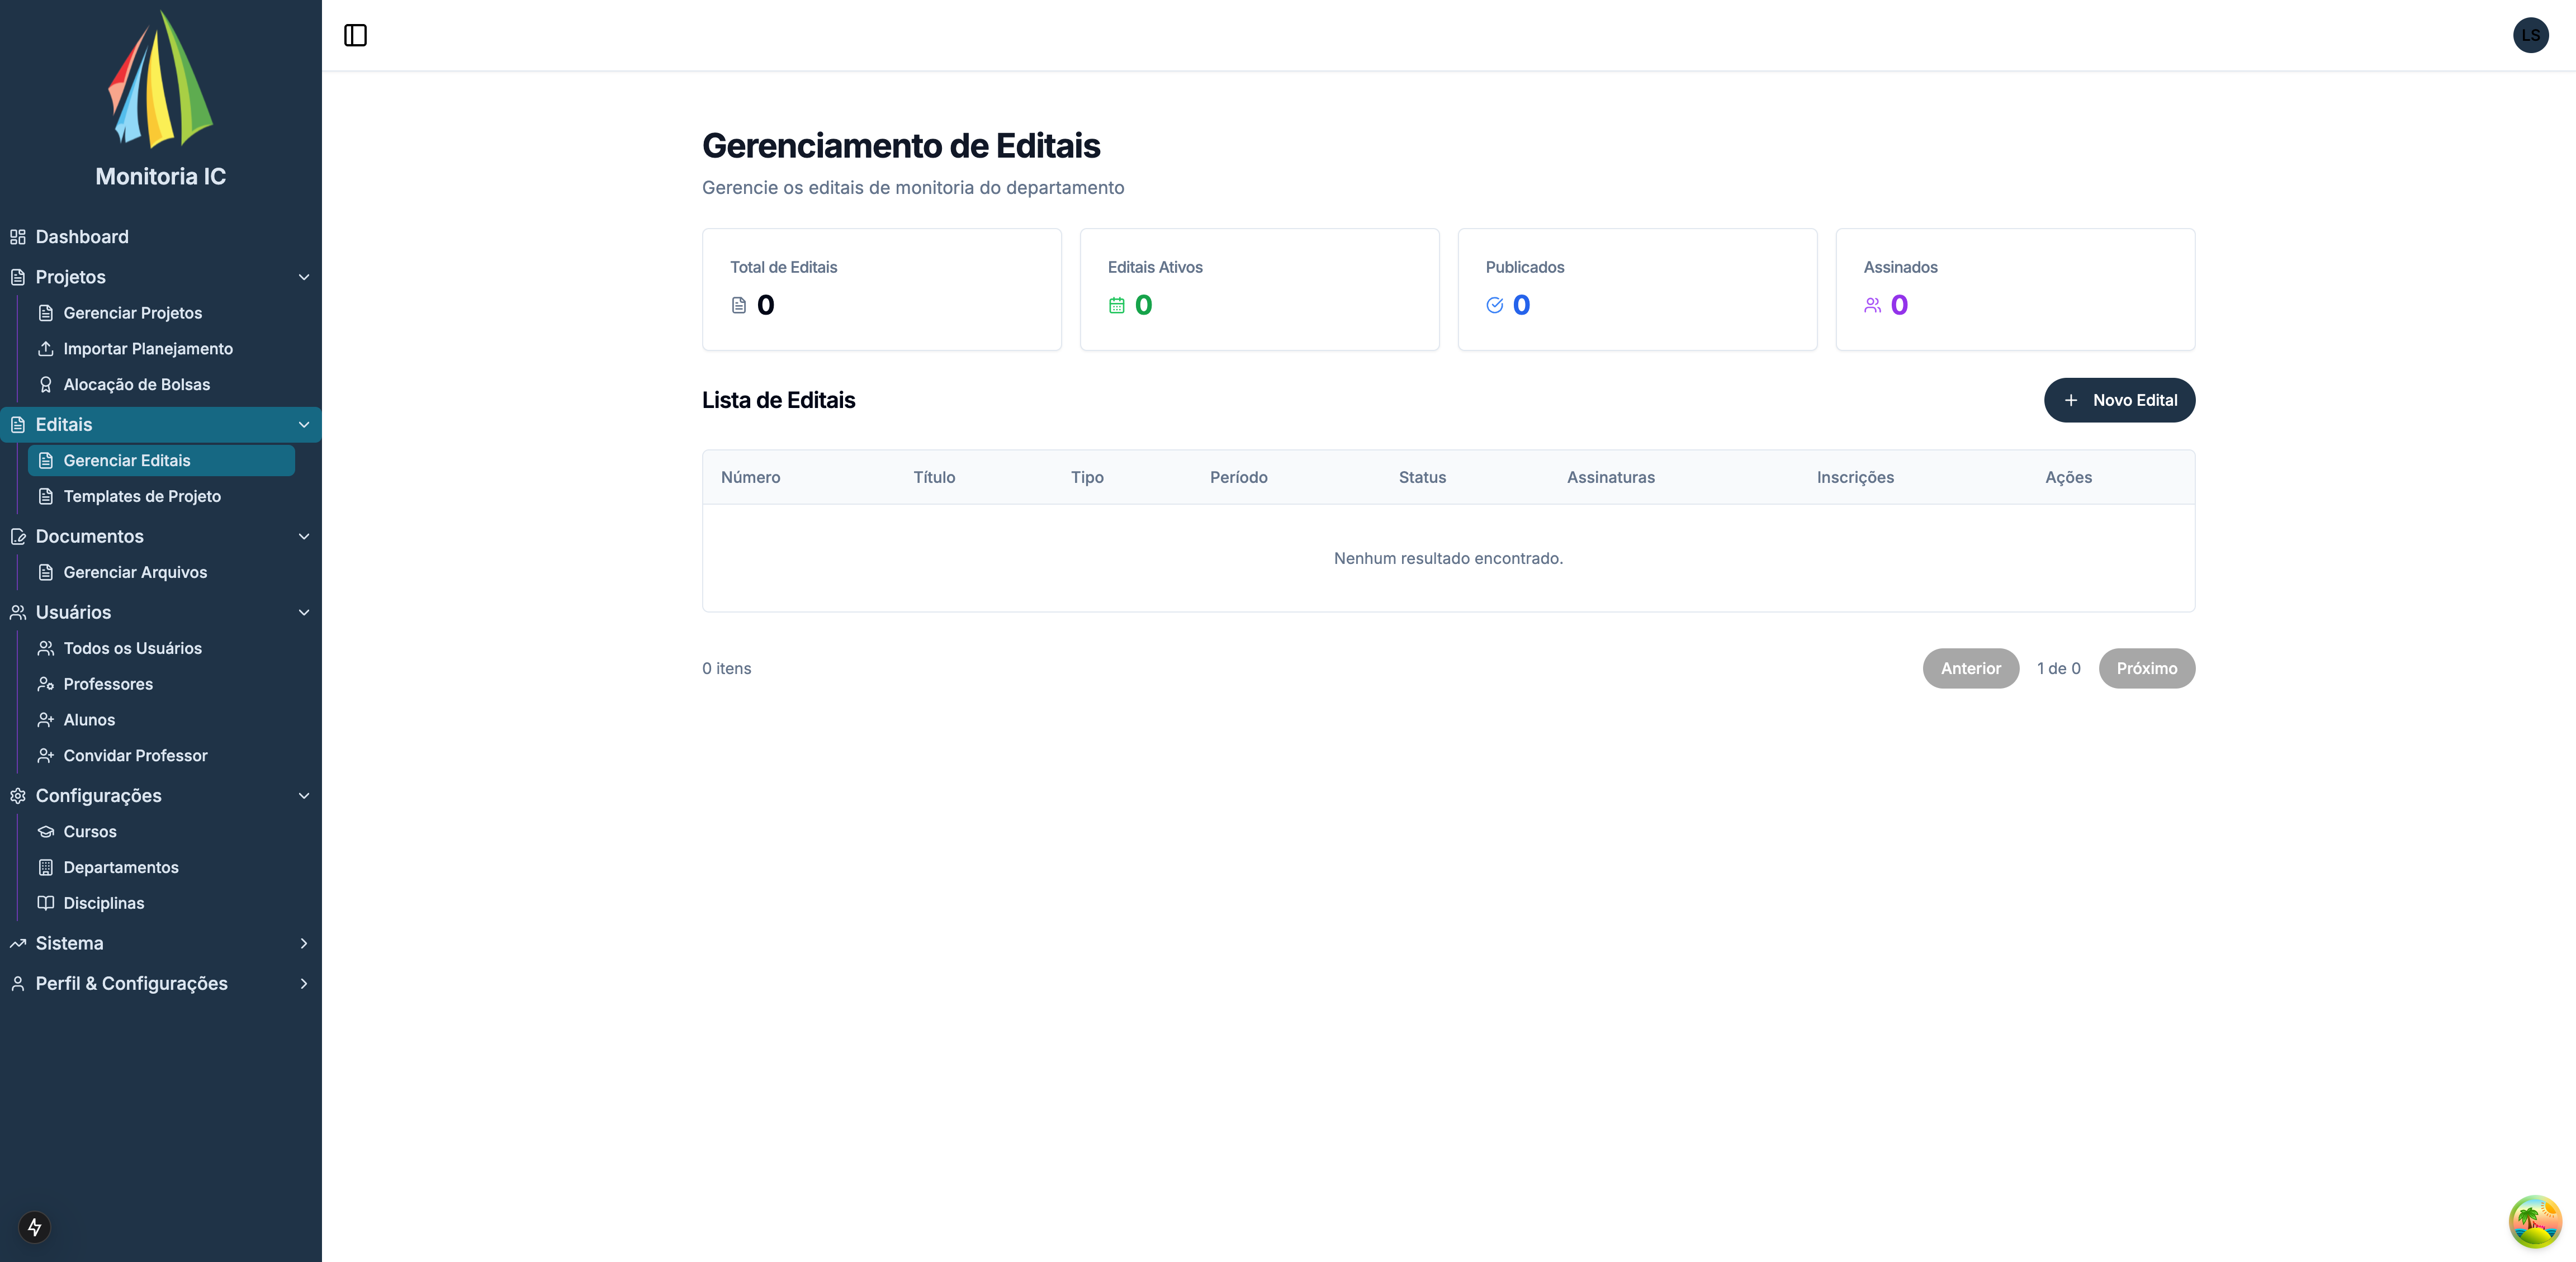
\includegraphics[width=\linewidth]{images/monitoria/admin-edital-management.png}
  \caption{Gestão de editais com status e ações}
  \label{fig:editais}
\end{figure}

\begin{figure}[h!]
  \centering
  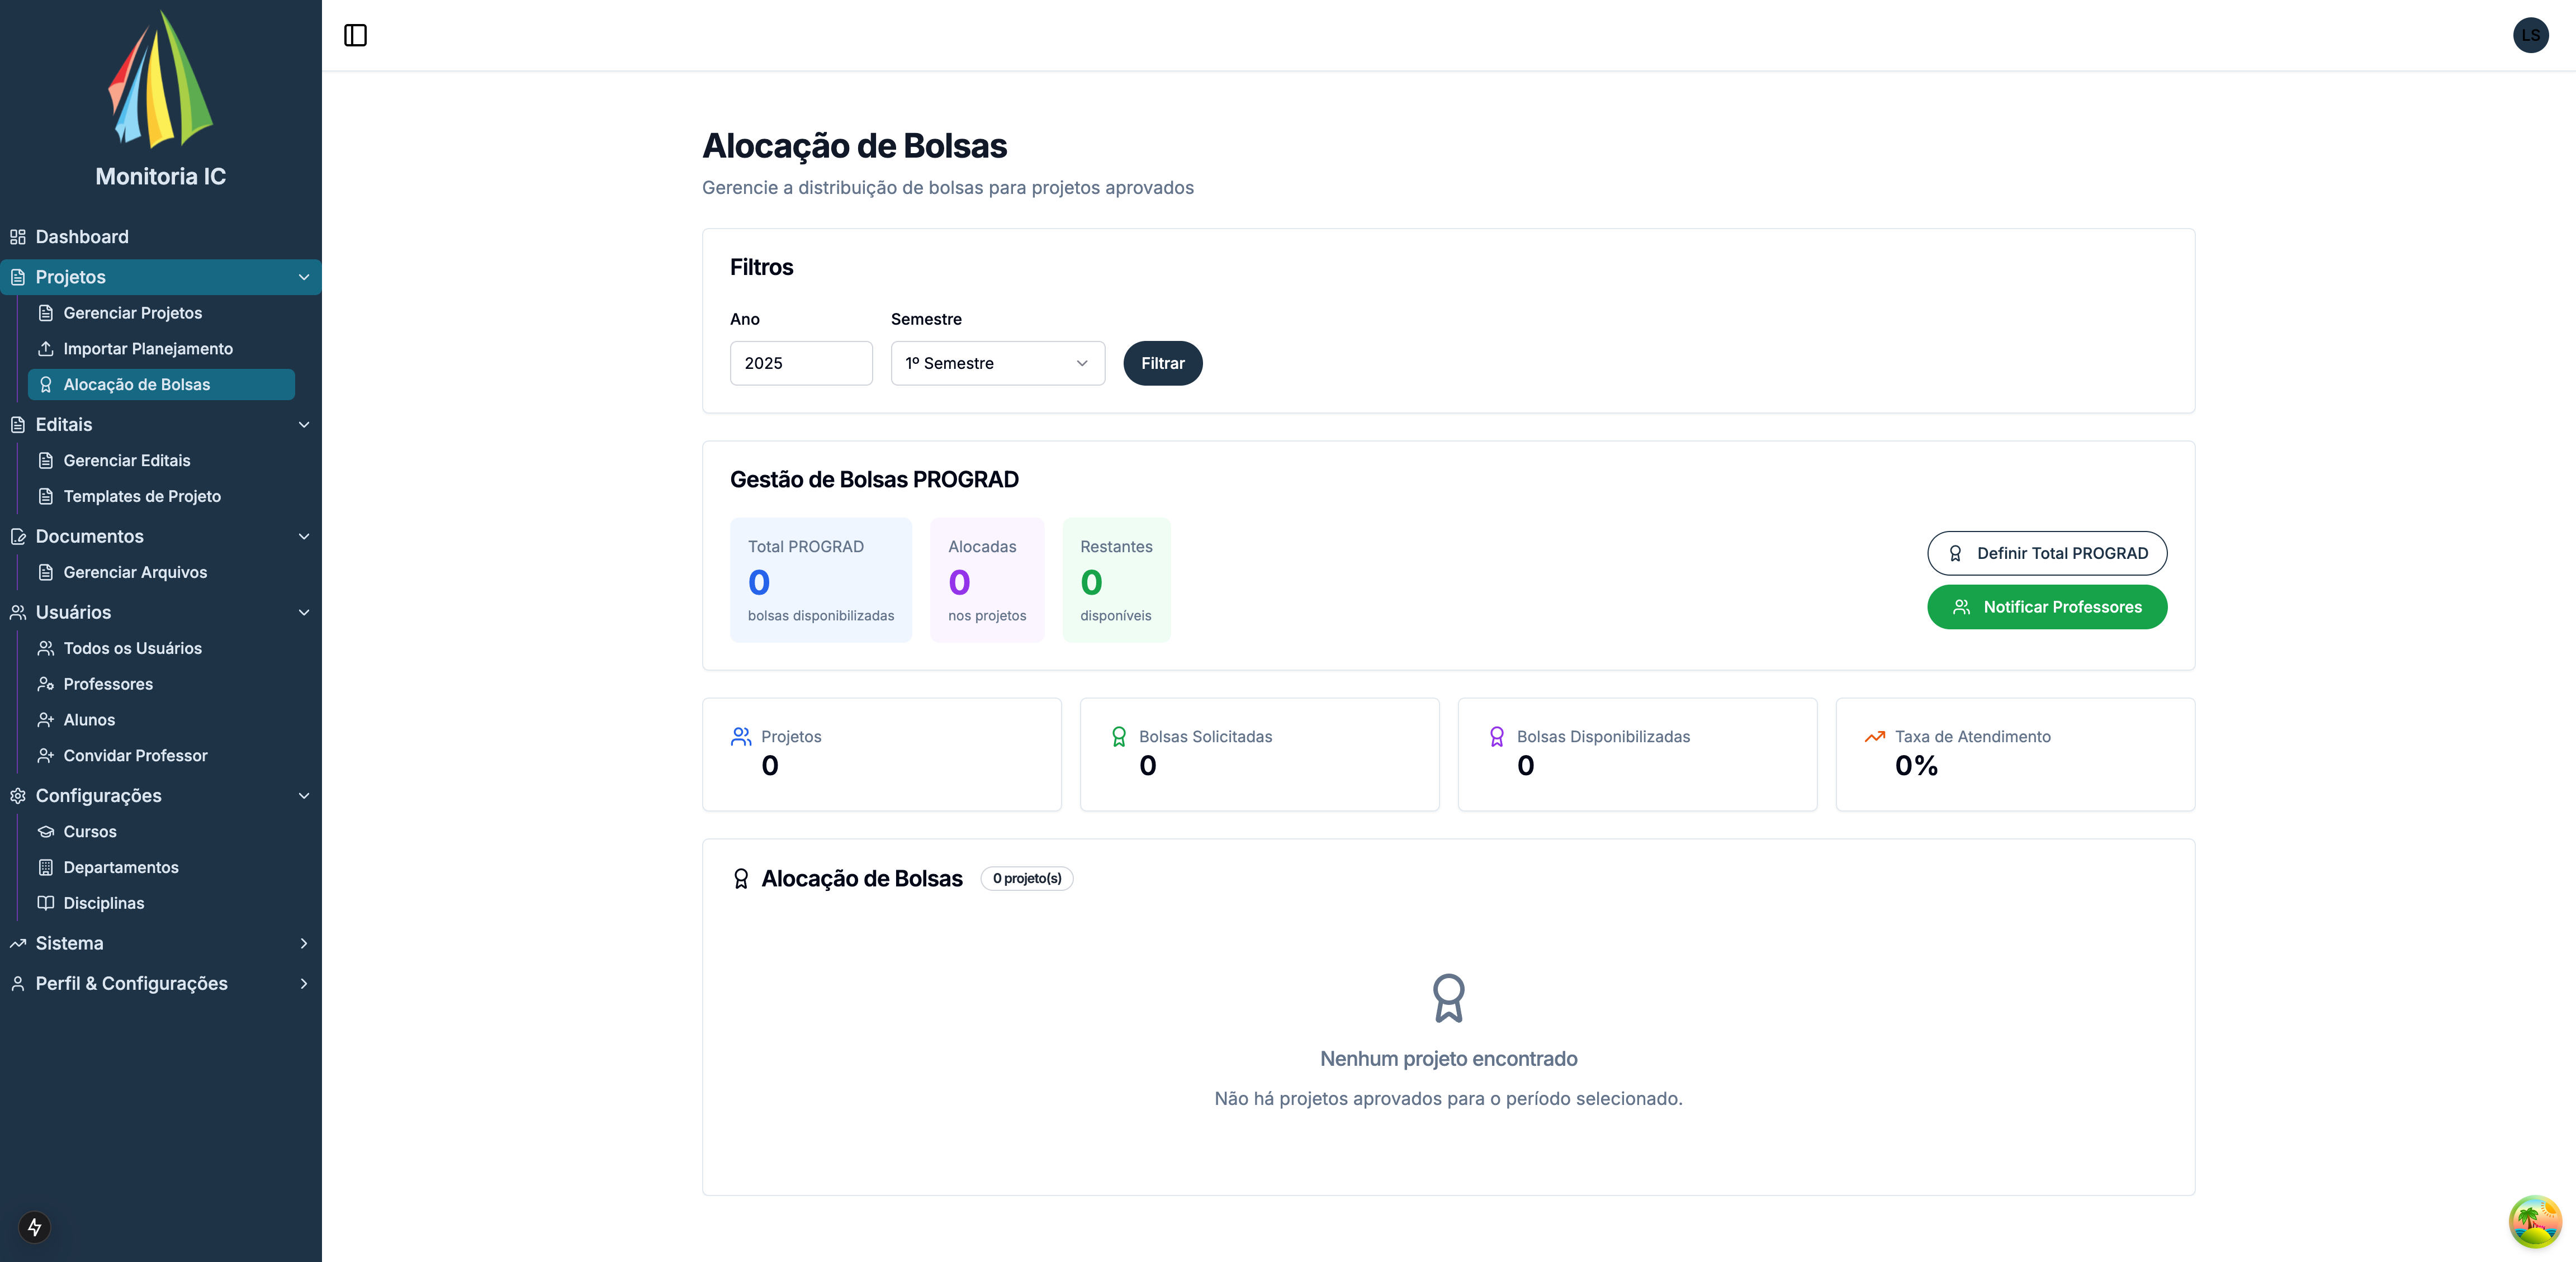
\includegraphics[width=\linewidth]{images/monitoria/admin-scholarship-allocation.png}
  \caption{Interface de alocação de bolsas}
  \label{fig:bolsas}
\end{figure}

\section{Resultados e Discussão}
\label{sec:results}

Esta seção apresenta os resultados obtidos com a implementação do Sistema de Monitoria-IC, incluindo análises quantitativas e qualitativas do impacto na gestão de monitorias do Instituto de Computação da UFBA.

\medskip
\noindent\textbf{Nota metodológica (TODO – Dados).} Alguns valores quantitativos reportados nesta seção (desempenho, adoção e comparação antes/depois) são \textit{preliminares} e serão substituídos por dados finais após a coleta sistemática com base em logs de produção, planilhas institucionais e questionários validados. A coleta e consolidação estatística compõem trabalho em andamento, e os números apresentados aqui devem ser interpretados como estimativas a serem confirmadas.

\subsection{Implantação e Ambiente de Produção}

O Sistema de Monitoria-IC está em produção desde janeiro de 2025 (\url{https://sistema-de-monitoria.app.ic.ufba.br/}) como plataforma oficial do Instituto de Computação. A infraestrutura é provisionada em servidor dedicado do datacenter institucional, com PostgreSQL 16 configurado para redundância, MinIO em cluster de três nós para armazenamento distribuído, Nginx como \textit{reverse proxy} com SSL e cache estático, além de monitoramento contínuo com Prometheus e Grafana. Políticas de backup incremental a cada seis horas (com diários completos e retenção de 30 dias) e entrega otimizada por CDN complementam a operação.

\subsection{Testes e Qualidade de Software}

A estratégia de qualidade combina testes unitários, de integração e end-to-end, integrados a uma pipeline de CI/CD. Com Vitest, 287 testes garantem 89\% de cobertura em lógica de negócio, executando em menos de 30 segundos. A camada de integração valida \textit{procedures} tRPC e operações de banco de dados sob transações, enquanto o Playwright automatiza 26 fluxos completos que cobrem os principais \textit{user journeys} em múltiplos navegadores. No GitHub Actions, a pipeline realiza linting e formatação (Biome), verificação de tipos (TypeScript), execução de testes unitários e de integração, build de produção, testes E2E em ambiente isolado e, após aprovação, \textit{deploy} automatizado.

\subsection{Métricas de Desempenho}

Em produção, as medições indicam tempo de carregamento inicial de 1,2 s (First Contentful Paint) e \textit{Time to Interactive} de 2,1 s, com pontuação Lighthouse de 96/100. A API mantém latência média de 45 ms e sustenta cerca de 500 requisições por segundo. No piloto de 2024.2 no Departamento de Ciência da Computação, foram cadastrados e gerenciados 152 projetos de monitoria, com 47 professores ativos (adesão integral), 823 inscrições processadas e 198 monitores selecionados (78 bolsistas e 120 voluntários), abrangendo 68 disciplinas e reutilizando 12 templates entre semestres.

Do ponto de vista operacional, observou-se redução aproximada de 85\% no tempo total de processamento administrativo, eliminação de erros de transcrição, conformidade integral com prazos institucionais e publicação de resultados cerca de três vezes mais rápida. O tempo médio de resposta a demandas administrativas passou para aproximadamente duas horas (cenário anterior: três a cinco dias).

\subsection{Análise de Impacto}

\subsubsection{Impacto Quantitativo}

\subsubsection{Antes vs Depois}

A Tabela \ref{tab:comparacao} compara métricas do processo manual anterior com o sistema implementado:

\begin{table*}[t]
  \centering
  \caption{Comparação entre processo manual e automatizado}
  \label{tab:comparacao}
  \begin{adjustbox}{max width=\textwidth}
    \begin{tabular}{|l|c|c|c|}
      \hline
      \textbf{Métrica} & \textbf{Manual} & \textbf{Sistema} & \textbf{Melhoria} \\
      \hline
      Criação de projeto & 2-3 dias & 30 min & 95\% \\
      Aprovação administrativa & 1 semana & 1 dia & 86\% \\
      Processamento de inscrições & 5 dias & Instantâneo & 100\% \\
      Consolidação de dados & 3 dias & 5 min & 99\% \\
      Geração de relatórios & 2 dias & Automático & 100\% \\
      Erros de preenchimento & 15\% & <1\% & 93\% \\
      Retrabalho administrativo & Alto & Mínimo & 90\% \\
      \hline
    \end{tabular}
  \end{adjustbox}
\end{table*}

\subsubsection{Benefícios Identificados}

Os ganhos quantitativos incluem economia estimada de 120 horas administrativas por semestre, redução de cerca de 95\% no uso de papel, eliminação de erros de transcrição e aumento aproximado de 40\% no volume de inscrições motivado pela simplificação do processo. Em termos qualitativos, a plataforma promove transparência \textit{end-to-end} com histórico auditável, padroniza processos entre departamentos, eleva a satisfação de professores e estudantes e cria uma base confiável para análises e tomada de decisão institucional.

\subsection{Feedback dos Usuários}

Em pesquisa com os primeiros usuários (n=73), 92\% avaliaram o sistema como “muito melhor” que o processo anterior, 88\% reportaram economia significativa de tempo e 95\% consideraram a interface intuitiva; entre administradores, a recomendação de expansão foi unânime. Os depoimentos reforçam os achados: “Finalmente posso reutilizar meus projetos anteriores”, “O processo de seleção ficou muito mais transparente”, “Não preciso mais verificar e-mails constantemente” e “A geração automática de documentos é fantástica”. Como oportunidades de evolução, destacaram-se um aplicativo móvel, notificações por WhatsApp além de e-mail, painéis personalizados por professor e exportações direcionadas para análises externas.

\section{Conclusão e Trabalhos Futuros}
\label{sec:conclusion}

\subsection{Contribuições Principais}

Este trabalho apresentou o desenvolvimento e a implantação do Sistema de Monitoria-IC como solução específica para o \textit{workflow} completo de monitoria. As contribuições centrais abrangem a automação integral de processos (da importação de dados à emissão de certificados), a adoção de uma arquitetura moderna e escalável que separa SPT e funcionalidades gerenciais, a validação em produção com métricas de eficiência e a disponibilização de uma base estruturada que viabiliza pesquisas sobre efetividade de programas de monitoria.

\subsection{Impacto Institucional}

A adoção do sistema produz efeitos mensuráveis no cotidiano administrativo, reduzindo significativamente o tempo gasto em tarefas repetitivas, eliminando retrabalho e padronizando procedimentos entre departamentos. Na dimensão estratégica, a consolidação de dados permite análises históricas e de tendências, qualificando a tomada de decisão e abrindo espaço para políticas institucionais orientadas por evidências. Do ponto de vista pedagógico, a maior facilidade de participação amplia o alcance do programa, a transparência reforça a confiança de todos os atores e a economia de tempo libera docentes para atividades-fim.

\subsection{Limitações Atuais}

Apesar dos resultados positivos, permanecem desafios: a integração com o sistema acadêmico ainda é parcial para captura automática de CR e histórico; o escopo atual está restrito ao Instituto de Computação, exigindo adaptações para expansão; parte do fluxo depende de setores externos (PROGRAD, NUMOP), o que mantém etapas manuais; e a ausência de um aplicativo móvel nativo pode limitar o acesso em determinados contextos.

\subsection{Trabalhos Futuros}

O plano de evolução contempla três horizontes. No curto prazo (seis meses), prioriza-se a conclusão da integração com o sistema acadêmico (SIAC), a entrega do módulo de certificados digitais, o desenvolvimento do aplicativo móvel (React Native) e a expansão controlada para outros departamentos da UFBA. No médio prazo (cerca de um ano), o foco recai sobre um sistema de recomendação para \textit{matching} aluno–projeto, analytics avançado com \textit{machine learning}, integrações com plataformas de ensino (como Moodle) e a disponibilização de uma API pública para sistemas terceiros. No longo prazo, busca-se generalizar o uso para outras universidades, criar um marketplace de templates entre instituições, conduzir estudos longitudinais sobre o impacto da monitoria e publicar o projeto como software livre para a comunidade acadêmica.

\subsection{Considerações Finais}

O Sistema de Monitoria-IC representa um avanço significativo na modernização da gestão acadêmica universitária. Ao digitalizar e automatizar processos tradicionalmente manuais, o sistema não apenas aumenta a eficiência operacional, mas também estabelece uma base sólida para a transformação digital contínua das universidades brasileiras.

A experiência de desenvolvimento e implantação deste sistema demonstra que é possível criar soluções tecnológicas específicas para problemas acadêmicos complexos, utilizando tecnologias modernas e práticas de engenharia de software consolidadas. O sucesso inicial na UFBA sugere alto potencial de replicação em outras instituições que enfrentam desafios similares.

Esperamos que este trabalho inspire outras iniciativas de modernização administrativa no ambiente universitário e contribua para o avanço da discussão sobre transformação digital na educação superior brasileira. O código fonte e documentação estarão disponíveis publicamente após a conclusão das funcionalidades principais, permitindo que outras instituições adaptem e evoluam a solução conforme suas necessidades específicas.

\section*{Agradecimentos}

Agradecemos ao Instituto de Computação da UFBA pelo apoio institucional, aos professores e alunos que participaram dos testes piloto, e à equipe de TI que viabilizou a infraestrutura necessária. Este trabalho foi parcialmente financiado por bolsa de iniciação científica do CNPq.

\bibliographystyle{apalike-sol}
\bibliography{references}

\end{document}